\documentclass[12pt,a4paper]{article}
\usepackage[UTF8]{ctex}     %先引入ctex
\usepackage[utf8]{inputenc} %再引入inputenc
\usepackage{graphicx}
% \usepackage{lazylatex}
% \tcbuselibrary{documentation}
\usepackage{multicol}
\usepackage{tikz}
\usetikzlibrary{matrix}
\usepackage{pgfplots}
\usepgfplotslibrary{colorbrewer}
\pgfplotsset{compat=1.17}
\usepackage{xcolor}
\usepackage{listings}
\usepackage{amsmath}
\usepackage{bookmark}
\usepackage{enumerate}
\usepackage{geometry}
\graphicspath{{img/}}
% 边距
\geometry{left=2.0cm,right=2.0cm,top=2.0cm,bottom=3.0cm}
% 大题
\newenvironment{problems}{\begin{list}{}{\renewcommand{\makelabel}[1]{\textbf{##1}.\hfil}}}{\end{list}}
% 小题
\newenvironment{steps}{\begin{list}{}{\renewcommand{\makelabel}[1]{(##1)\hfil}}}{\end{list}}
% 答
\providecommand{\ans}{\textbf{答}:~}
% 解
\providecommand{\sol}{\textbf{解}.~}

% \setminted{breaklines,autogobble,frame=lines,framesep=2mm,fontsize=\scriptsize}

% listings
\definecolor{grey}{rgb}{0.8,0.8,0.8}
\definecolor{darkgreen}{rgb}{0,0.3,0}
\definecolor{darkblue}{rgb}{0,0,0.3}
\lstset{%
    numbers=left, %行号
    numberstyle=\tiny\color{grey},
    showstringspaces=false,
    showspaces=false,%
    tabsize=4,%
    frame=shadowbox,%
    basicstyle={\ttfamily\scriptsize},%
    keywordstyle=\color{blue!80!black}\bfseries,%
    commentstyle=\color{green!50!blue}\itshape,%
    stringstyle=\color{green!50!black},%
    rulesepcolor=\color{gray!20!white},
    breaklines,
    columns=flexible,
    extendedchars=false,
    %mathescape=true,
    language=c,
}

\setlength{\columnsep}{3em}

\begin{document}
\title{\normalsize \underline{计算机系统结构(A)}\\\LARGE 实验 5}
\author{Log Creative }
\date{\today}
\maketitle

\begin{problems}
    \item[一] \textbf{熟悉 SIMD intrinsics 函数}
    \begin{itemize}
        \item 4 个并行的单精度浮点数除法
        \begin{lstlisting}[identifierstyle=\color{blue}]
            __m128 _mm_div_ps (__m128 a, __m128 b)
        \end{lstlisting}
        \item 16 个并行求8 位无符号整数的最大值
        \begin{lstlisting}[identifierstyle=\color{blue}]
            __m128i _mm_max_epi16 (__m128i a, __m128i b)
        \end{lstlisting}
        \item 8 个并行的16 位带符号短整数的算术右移
        \begin{lstlisting}[identifierstyle=\color{blue}]
            __m128i _mm_bsrli_si128 (__m128i a, int imm8)
        \end{lstlisting}
    \end{itemize}
    \item[二] \textbf{阅读SIMD代码}
    仅关注函数的主要部分,执行 SIMD 操作的行用 \verb";SIMD" 标识。
    \lstset{language=[x86masm]Assembler}
	\begin{multicols}{2}
		\begin{lstlisting}
.LFB5548:
	.cfi_startproc
	endbr64
	sub	rsp, 120
	.cfi_def_cfa_offset 128
	pxor	xmm6, xmm6
	movsd	xmm1, QWORD PTR .LC2[rip]			;SIMD
	movsd	xmm10, QWORD PTR .LC0[rip]			;SIMD
	mov	rax, QWORD PTR fs:40
	mov	QWORD PTR 104[rsp], rax
	xor	eax, eax
	mov	rax, QWORD PTR .LC3[rip]
	movsd	xmm8, QWORD PTR .LC1[rip]			;SIMD
	mov	QWORD PTR 64[rsp], 0x000000000
	movsd	QWORD PTR 48[rsp], xmm1				;SIMD
	pxor	xmm9, xmm9
	lea	rsi, .LC6[rip]
	mov	edi, 1
	mov	QWORD PTR 56[rsp], rax
	movapd	xmm0, XMMWORD PTR 48[rsp]			;SIMD
	movapd	xmm3, xmm9							;SIMD
	mov	eax, 6
	movsd	QWORD PTR 32[rsp], xmm10			;SIMD
	movapd	xmm2, xmm0							;SIMD
	movsd	QWORD PTR 40[rsp], xmm8				;SIMD
	movapd	xmm7, XMMWORD PTR 32[rsp]			;SIMD
	addpd	xmm0, xmm0							;SIMD
	mov	QWORD PTR 72[rsp], 0x000000000
	mulpd	xmm2, xmm6							;SIMD
	mov	QWORD PTR 80[rsp], 0x000000000
	mulpd	xmm6, XMMWORD PTR 32[rsp]			;SIMD
	mulpd	xmm7, XMMWORD PTR .LC5[rip]			;SIMD
	mov	QWORD PTR 88[rsp], 0x000000000
	addpd	xmm7, XMMWORD PTR 64[rsp]			;SIMD
	addpd	xmm6, XMMWORD PTR 80[rsp]			;SIMD
	addpd	xmm7, xmm2							;SIMD
	addpd	xmm6, xmm0							;SIMD
	movapd	xmm2, xmm1							;SIMD
	movapd	xmm0, xmm10							;SIMD
	movapd	xmm5, xmm6							;SIMD
	movapd	xmm4, xmm7							;SIMD
	movaps	XMMWORD PTR 16[rsp], xmm6			;SIMD
	movaps	XMMWORD PTR [rsp], xmm7				;SIMD
	call	__printf_chk@PLT
	movapd	xmm6, XMMWORD PTR 16[rsp]			;SIMD
	movapd	xmm7, XMMWORD PTR [rsp]				;SIMD
	pxor	xmm9, xmm9
	mov	rax, QWORD PTR .LC1[rip]	
	movapd	xmm2, xmm9							;SIMD
	mov	edi, 1	
	lea	rsi, .LC7[rip]
	unpckhpd	xmm6, xmm6						;SIMD
	unpckhpd	xmm7, xmm7						;SIMD
	movq	xmm8, rax
	movq	xmm3, rax
	mov	rax, QWORD PTR .LC3[rip]
	movapd	xmm5, xmm6							;SIMD
	movapd	xmm4, xmm7							;SIMD	
	movapd	xmm0, xmm8							;SIMD
	movq	xmm1, rax
	mov	eax, 6
	call	__printf_chk@PLT
	mov	rax, QWORD PTR 104[rsp]
	xor	rax, QWORD PTR fs:40
	jne	.L5
	xor	eax, eax
	add	rsp, 120
	.cfi_remember_state
	.cfi_def_cfa_offset 8
	ret
    \end{lstlisting} 
	\end{multicols}
    
	\item[三] \textbf{书写 SIMD 代码}
	
	函数 \verb"sum_vectorized()" 的实现如下。
	
	\begin{lstlisting}[language=c]
static int sum_vectorized(int n, int *a)
{
    // WRITE YOUR VECTORIZED CODE HERE

	// the parallelization could only
	// apply on aligned groups
	int groups =  n / 4;

	// On linux, int is 32-bit wide.
	// 128-bit = 4 int;
	// Initialize sum vector of 128-bit as zero.
	__m128i sum = _mm_setzero_si128();

	// For loop will add numbers on mod 4 basis.
	for(int i = 0; i < groups; ++i){
		// load a vector of adders.
		__m128i adder = _mm_loadu_si128(a + i * 4);

		// add the vector to a temporary variable.
		__m128i added = _mm_add_epi32(sum, adder);

		// store the value to the sum vector.
		_mm_storeu_si128(&sum, added);
	}

	int result = 0;

	// However there is some remaining numbers
	// that didn't count, whose quantity is < 4.
	int remain = n - groups * 4;
	int tip = groups * 4;

	// For each offset, calulate manually.
	for(int j = 0; j < remain; ++j)
		result += a[tip++];

	// and to get the final result, the member
	// of the vector in sum has to be added as well,
	// in other word, 4 numbers.
	
	// For each right shift, get the lower 32 bit.
	// which is one unit and add to the result.
	for(int i = 0; i < 4; ++i)
		result += _mm_cvtsi128_si32(_mm_srli_si128(sum,i * 4));

    return result;
}
	\end{lstlisting}

	第一轮测评性能得到了改善(提升了 236\%),输出结果如下:
	\begin{figure}[h]
		\centering
		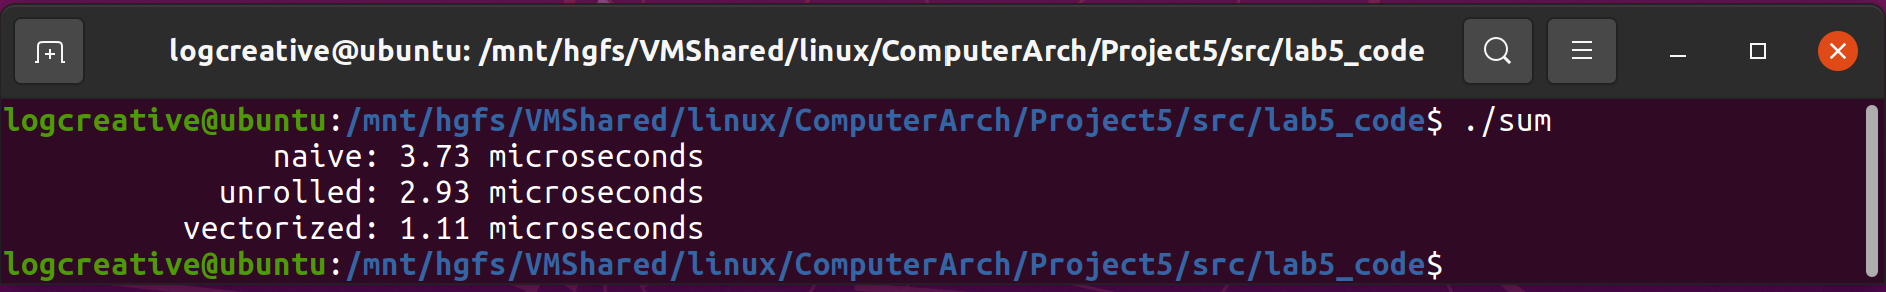
\includegraphics[width=\textwidth]{benchmark1.png}
	\end{figure}
	
	\item[四] \textbf{循环展开}
	
	函数 \verb"sum_vectorized_unrolled()" 的实现如下:
	\begin{lstlisting}[language=c]
static int sum_vectorized_unrolled(int n, int *a)
{
    // UNROLL YOUR VECTORIZED CODE HERE

	__m128i sum = _mm_setzero_si128();

	// For unrolled scenario,
	// every loop will contribute 128 * 4 = 512 bit operation.
	for(int i = 0; i < n / 16 * 16; i += 16){
		_mm_storeu_si128(&sum, _mm_add_epi32(sum, _mm_loadu_si128(a + i )));
		_mm_storeu_si128(&sum, _mm_add_epi32(sum, _mm_loadu_si128(a + i + 4)));
		_mm_storeu_si128(&sum, _mm_add_epi32(sum, _mm_loadu_si128(a + i + 8)));
		_mm_storeu_si128(&sum, _mm_add_epi32(sum, _mm_loadu_si128(a + i + 12)));
	}
	
	int result = 0;
	for(int i = n / 16 * 16; i < n; i++)
		result += a[i];
	
	for(int k = 0; k < 4; ++k)
		result += _mm_cvtsi128_si32(_mm_srli_si128(sum,k * 4));

    return result;
}
	\end{lstlisting}

	第二轮测评结果也得到了改善(提升了 274\%),输出结果如下:
	\begin{figure}[h]
		\centering
		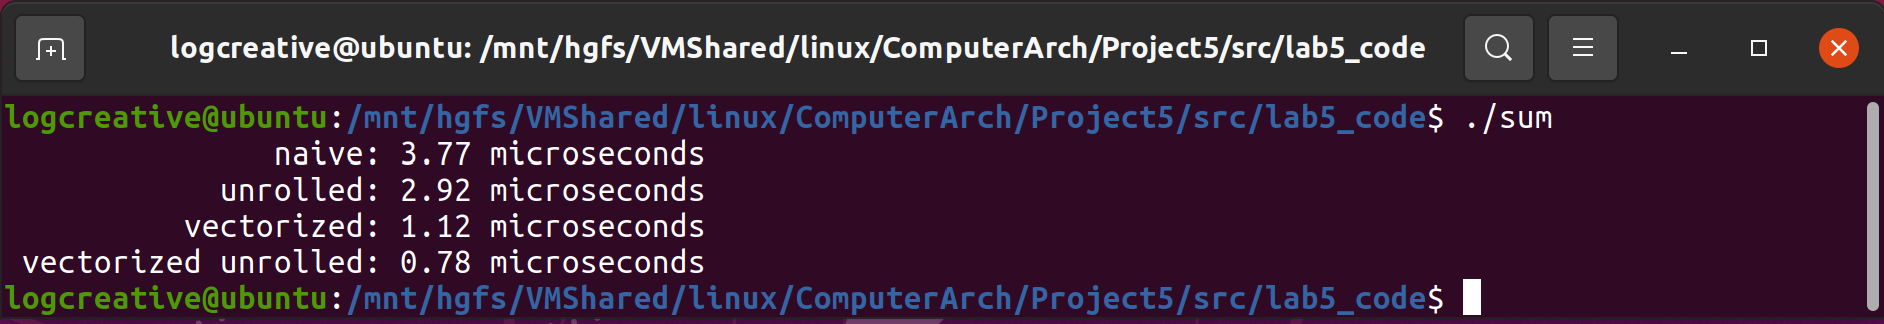
\includegraphics[width=\textwidth]{benchmark2.png}
	\end{figure}

	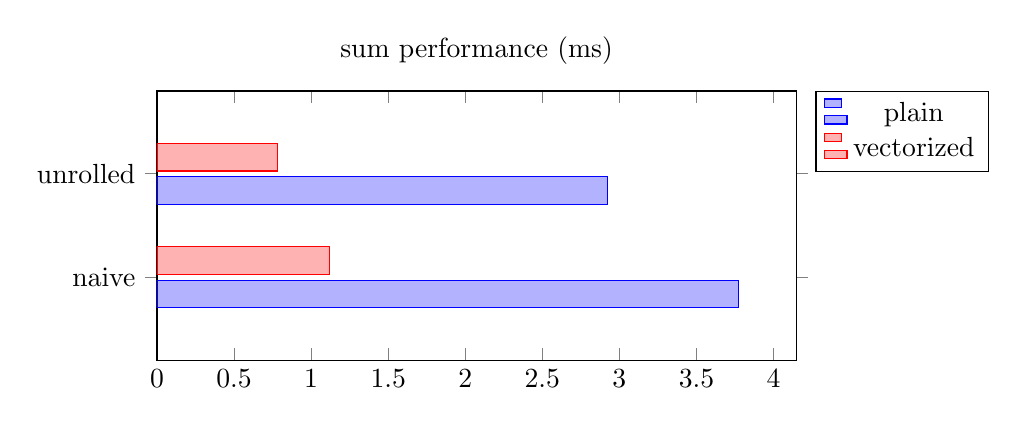
\begin{tikzpicture}
		\begin{axis}[width=0.8\textwidth,
		height={5cm},
		xmin={0},
		legend pos={outer north east},
		title={sum performance (ms)},
		symbolic y coords={naive, unrolled},xbar,enlarge y limits=0.8,]
		 \addplot+ [] coordinates { (3.77,naive) (2.92,unrolled)};
		 \addplot+ [] coordinates { (1.12,naive) (0.78,unrolled)};
		 \legend{plain,vectorized,}
		\end{axis}
		\end{tikzpicture}		

\end{problems}
\end{document}
